\documentclass[conference,a4paper]{IEEEtran}
\usepackage[T1]{fontenc}
\usepackage[utf8]{inputenc}
\usepackage[brazil]{babel}
\usepackage{lmodern}
\usepackage{amsmath,amssymb,booktabs,graphicx,microtype}
\usepackage{xurl}
\usepackage[hidelinks]{hyperref}
\usepackage{listings,xcolor}
\hyphenation{Best-First}
\lstdefinestyle{pytrecho}{
 language=Python,basicstyle=\ttfamily\scriptsize,
 frame=single,framerule=.3pt,rulecolor=\color{black!35},
 backgroundcolor=\color{black!3},
 aboveskip=3pt,belowskip=3pt,
 xleftmargin=2pt,xrightmargin=2pt,
 breaklines=true,breakatwhitespace=true,
 showstringspaces=false,columns=fullflexible,keepspaces=true,
 tabsize=4
}
\lstset{style=pytrecho}
\title{Mini-Projeto: Buscas Clássicas e Otimização Contínua}
\author{\IEEEauthorblockN{Luan Diniz Mazaro Rodovalho}
\IEEEauthorblockA{Universidade Federal de Uberlândia (UFU)\\Brasil}}
\begin{document}
\maketitle

\begin{abstract}
Este trabalho apresenta a implementação e a avaliação de métodos de busca em espaço discreto e de otimização contínua aplicados à transformação de sequências binárias. Na primeira etapa, foram desenvolvidas uma busca em largura (BFS), uma busca gulosa \textit{Best-First} e uma variante gulosa que explora a estrutura dos intervalos de bits. Na segunda etapa, foi implementado o gradiente descendente projetado, com posterior inclusão de uma penalidade para alterações não consecutivas. Os experimentos utilizaram 30 pares aleatórios para cada comprimento entre 2 e 4096 bits; em razão do crescimento combinatório, as buscas com enumeração explícita foram avaliadas apenas até 16 bits.
\end{abstract}
\begin{IEEEkeywords}
Busca em largura, busca gulosa, sequências binárias, gradiente descendente, otimização.
\end{IEEEkeywords}

\section{Modelagem do Problema e Operações de Flip}
O problema inicial consistiu em transformar uma sequência binária $s\in\{0,1\}^L$ em outra sequência $t$ do mesmo comprimento. Para isso, foram consideradas duas operações: a inversão de um único bit e a inversão de um intervalo de bits consecutivos. Ambas receberam custo unitário, independentemente do número de posições modificadas. A operação sobre um intervalo inclusivo $[i,j]$ foi formalizada por
\begin{equation}
F_{i,j}(s)_k=\begin{cases}1-s_k,&i\leq k\leq j,\\s_k,&\text{caso contrário.}\end{cases}
\end{equation}

Foram implementadas as funções \texttt{flip\_bit} e \texttt{flip\_intervalo}, com verificação dos limites dos índices e da validade da sequência. A primeira reutilizou a segunda, especificando um intervalo de apenas uma posição. No trecho a seguir, observa-se a construção da nova sequência por concatenação da parte anterior, do intervalo invertido e da parte posterior.
\begin{lstlisting}
def flip_bit(estado: str, pos: int) -> str:
    return flip_intervalo(estado, pos, pos)
\end{lstlisting}
\begin{lstlisting}
pre = estado[:inicio-1]
mid = ''.join('1' if c == '0' else '0' for c in estado[inicio-1:fim])
return pre + mid + estado[fim:]
\end{lstlisting}

A identificação das posições a modificar foi realizada por meio da diferença binária $d=s\oplus t$. Nessa representação, cada bit igual a 1 indicou uma divergência em relação ao estado-alvo. A análise dos blocos máximos de 1 também fundamentou a heurística e a posterior interpretação do custo ótimo.

\section{Implementação das Buscas Clássicas}
\subsection{Busca em largura (BFS)}
A BFS foi implementada com uma fila FIFO, iniciada pelo estado de origem. Cada estado removido da fila foi expandido mediante a geração de todos os $L(L+1)/2$ intervalos possíveis. Para representar as inversões, foram construídas máscaras binárias aplicadas ao estado por XOR. Cada estado descoberto recebeu um predecessor e a operação utilizada, permitindo reconstruir o caminho após a identificação do objetivo. O trecho central da expansão foi:
\begin{lstlisting}
for mask, op in masks:
    gerados += 1
    vizinho = atual ^ mask
    if vizinho not in pais:
        pais[vizinho] = atual, op
        fila.append(vizinho)
\end{lstlisting}

Como todas as arestas representaram operações de custo 1, a primeira trajetória encontrada pela BFS até o objetivo teve custo mínimo. Entretanto, o grafo possui $2^L$ estados possíveis e cada expansão pode examinar $O(L^2)$ intervalos. Consequentemente, o tempo no pior caso é $O(2^L L^2)$, com armazenamento potencial de $O(2^L)$ estados e seus predecessores. Essa característica motivou a restrição do experimento a comprimentos computacionalmente viáveis.

\subsection{Busca gulosa e heurística}
Para orientar a busca gulosa, foi definida uma heurística baseada na quantidade de blocos máximos de 1 na diferença entre o estado corrente e o objetivo:
\begin{equation}
\boxed{h(s)=\#\{\text{blocos de 1 em }s\oplus t\}.}
\end{equation}
A implementação contou os blocos por meio das funções \texttt{diferencas} e \texttt{blocos\_um}:
\begin{lstlisting}
def heuristica(estado: str, alvo: str) -> int:
    return len(blocos_um(diferencas(estado, alvo)))
\end{lstlisting}

Essa escolha foi justificada pela relação entre blocos e inversões. Acrescentando zeros às extremidades de $d$, um conjunto de $r$ blocos apresenta $2r$ transições entre 0 e 1. Uma inversão de intervalo modifica apenas as transições em suas extremidades e, portanto, reduz a quantidade de blocos em no máximo uma unidade. Assim, qualquer solução requer pelo menos $r$ operações. Por outro lado, a inversão individual de cada bloco alcança o objetivo em exatamente $r$ operações. Desse modo, foi estabelecido que $h(s)=r$ corresponde ao custo ótimo restante.

Na versão \textit{Best-First}, os estados foram armazenados em uma fila de prioridade, ordenada exclusivamente por $h$. Também foi desenvolvida uma versão gulosa otimizada, que dispensou a enumeração dos vizinhos e selecionou diretamente os intervalos associados aos blocos identificados:
\begin{lstlisting}
d = diferencas(inicial, alvo)
caminho = blocos_um(d)
\end{lstlisting}
O levantamento desses intervalos exigiu uma única varredura da sequência, com complexidade $O(L)$ para a construção do caminho representado por pares de índices. A versão otimizada preservou o custo ótimo, mas não foi considerada equivalente à busca \textit{Best-First} convencional quanto ao número de estados explorados.

\subsection{Aplicação ao exemplo do enunciado}
As implementações foram examinadas utilizando a sequência inicial \texttt{00001001000011001100111} e o objetivo \texttt{00000000000000000000000}. A diferença entre as sequências apresentou cinco blocos: $[5,5]$, $[8,8]$, $[13,14]$, $[17,18]$ e $[21,23]$, considerando índices iniciados em 1. A inversão sucessiva desses intervalos produziu o estado desejado com \textbf{custo total igual a 5}. O resultado foi obtido pela versão gulosa otimizada e corresponde ao ótimo demonstrado pela propriedade dos blocos.

\section{Metodologia e Resultados das Buscas}
A avaliação experimental foi organizada em 12 comprimentos, $L\in\{2,4,8,\ldots,4096\}$. Para cada comprimento, foram gerados $N=30$ pares independentes de sequências com bits equiprováveis, utilizando o gerador do NumPy com semente 2026. Foram registrados o custo encontrado, o tempo de execução, a quantidade de estados expandidos e o número de sucessores gerados. O tempo foi medido com \texttt{time.perf\_counter}, e os dados individuais foram exportados para arquivos CSV.

Os testes com buscas convencionais foram limitados após a análise de seu custo computacional. Em $L=16$, a BFS gerou, em média, 3,8 milhões de sucessores por par, com tempo de 280 ms. Tanto a BFS quanto a \textit{Best-First} enumeram $L(L+1)/2$ intervalos por estado expandido: em $L=2^{12}=4096$, seriam $8.390.656$ candidatos \emph{em uma única expansão}. A BFS ainda enfrenta crescimento exponencial dos estados visitados; a \textit{Best-First}, embora mais seletiva, repetiria a geração de milhões de vizinhos ao longo do caminho. Por esses motivos, fixou-se $L=16$ como limite comum das buscas explícitas, sem pressupor que a \textit{Best-First} fosse inviável em todos os tamanhos intermediários. Para comprimentos maiores, foi executada a versão otimizada, que identifica os blocos em $O(L)$ sem gerar vizinhos. As três versões coincidiram no custo nos tamanhos compartilhados. Na Tabela~\ref{tab:busca}, ``--'' significa experimento não executado, e não tempo nulo.

\begin{table}[htbp]
\centering
\caption{Resultados médios de 30 pares por tamanho; tempos em ms.}
\label{tab:busca}
\scriptsize\setlength{\tabcolsep}{2.5pt}
\begin{tabular}{rrrrr}
\toprule
$L$ & Custo & BFS & Gulosa & Otimizada\\
\midrule
2    & 0,90    & 0,0021 & 0,0072 & 0,0012\\
4    & 1,13    & 0,0062 & 0,0216 & 0,0013\\
8    & 2,47    & 0,3091 & 0,1683 & 0,0018\\
16   & 4,00    & 280,382 & 1,3750 & 0,0032\\
32   & 8,23    & -- & -- & 0,0048\\
64   & 15,73   & -- & -- & 0,0070\\
128  & 32,83   & -- & -- & 0,0136\\
256  & 63,27   & -- & -- & 0,0287\\
512  & 128,10  & -- & -- & 0,0522\\
1024 & 257,93  & -- & -- & 0,1130\\
2048 & 512,57  & -- & -- & 0,2111\\
4096 & 1027,77 & -- & -- & 0,4070\\
\bottomrule
\end{tabular}
\end{table}

Os dados mostraram um aumento expressivo do trabalho realizado pela BFS. Para $L=16$, a busca expandiu, em média, $28.349{,}53$ estados e gerou $3.855.400{,}53$ sucessores, enquanto a \textit{Best-First} expandiu 5 estados e gerou 544 sucessores. A Figura~\ref{fig:tempo} apresenta os tempos medidos, evidenciando a diferença entre a expansão explícita do grafo e o processamento direto dos blocos.
\begin{figure}[htbp]
\centering
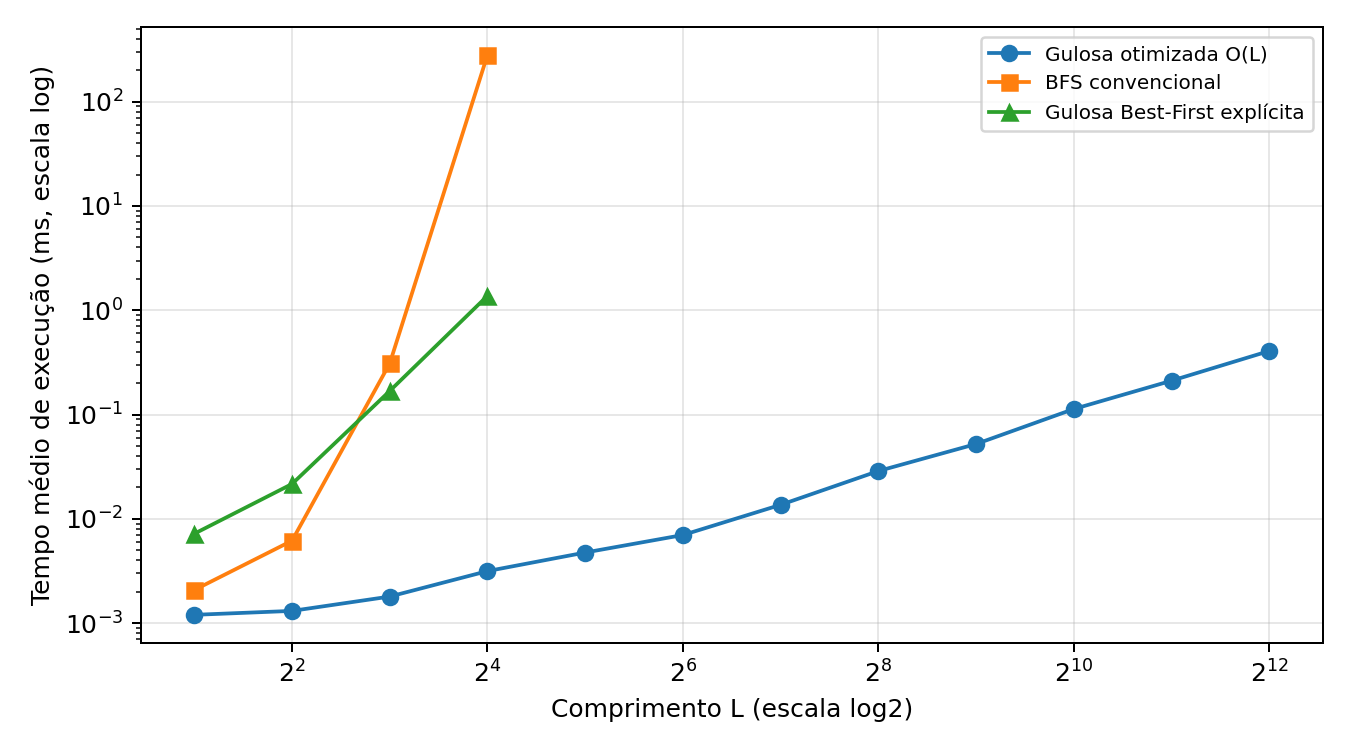
\includegraphics[width=\columnwidth]{resultados/grafico_tempo.png}
\caption{Tempo médio de execução em função do comprimento.}
\label{fig:tempo}
\end{figure}

A quantidade média de operações aumentou com o comprimento das sequências, em concordância com $\mathbb{E}[h]=(L+1)/4$ para pares independentes com bits equiprováveis. Acima de $L=16$, os custos foram calculados exclusivamente pela versão otimizada, cuja otimalidade foi demonstrada analiticamente.

\section{Otimização por Gradiente Descendente}
\subsection{Representação contínua e função erro}
Na segunda parte, cada bit foi representado por uma variável contínua $x_i\in[0,1]$. O vetor binário inicial foi denominado $x^{(0)}$ e o estado-alvo foi representado por $y$. Inicialmente, foi utilizada a função de erro quadrático proposta no enunciado:
\begin{equation}
\mathcal{L}(x)=\sum_{i=1}^L(x_i-y_i)^2,
\qquad \nabla\mathcal{L}(x)=2(x-y).
\end{equation}
A minimização dessa função aproxima cada coordenada do valor-alvo, sem impor preferência por modificações em posições consecutivas. A atualização do método sem penalidade foi expressa por
\begin{equation}
x^{(k+1)}=x^{(k)}-2\eta\bigl(x^{(k)}-y\bigr).
\end{equation}

Foram armazenadas as diferenças $\Delta x^{(k)}=x^{(k+1)}-x^{(k)}$ para representar as transformações contínuas entre iterações. Como valores fora de $[0,1]$ não correspondem à interpretação adotada para os bits, foi incorporada uma projeção por \texttt{np.clip}. O núcleo da implementação foi:
\begin{lstlisting}
novo_x = np.clip(x - eta*gradiente(x,x0,y,lam), 0., 1.)
passo = novo_x - x
passos.append(passo)
x = novo_x
\end{lstlisting}

O comportamento sem projeção também foi analisado. Para $x_i^{(0)}=1$, $y_i=0$ e $\eta=0{,}75>1/2$, a primeira atualização seria $x_i^{(1)}=1-2(0{,}75)=-0{,}5$, o que demonstra a possibilidade de saída do intervalo de validade. A projeção evitou esse comportamento nas execuções realizadas.

\subsection{Penalidade de adjacência e regra da cadeia}
Para representar o grau de alteração de cada posição, foi definido o peso de \textit{flip} $z_i$. A transformação dependeu do bit inicial, de modo que uma alteração completa tivesse peso 1 e a ausência de alteração tivesse peso 0:
\begin{equation}
 z_i=a_i(x_i-x_i^{(0)}), \quad a_i=1-2x_i^{(0)},
\end{equation}
\vspace{-.8em}
\begin{equation}
z_i=\begin{cases}x_i,&x_i^{(0)}=0,\\1-x_i,&x_i^{(0)}=1.\end{cases}
\end{equation}

Em seguida, foi proposta uma penalidade quadrática para diferenças entre pesos de posições vizinhas. Foram introduzidos valores artificiais nulos nas extremidades, $z_0=z_{L+1}=0$, resultando em
\begin{equation}
\boxed{C(z)=\sum_{i=0}^{L}(z_{i+1}-z_i)^2}, \quad
J(x)=\mathcal{L}(x)+\lambda C(z(x)).
\end{equation}
Essa construção favoreceu regiões contíguas com pesos semelhantes. No caso binário, cada bloco de posições alteradas produz duas transições e contribui com duas unidades para $C(z)$; no domínio contínuo, a penalidade constitui uma aproximação diferenciável desse comportamento. A função foi implementada da seguinte forma:
\begin{lstlisting}
zw = np.pad(z, (1,1), constant_values=0.)
return float(np.sum(np.diff(zw)**2))
\end{lstlisting}

A derivada da nova função objetivo foi obtida pela regra da cadeia. Como cada $z_i$ participa das parcelas referentes aos dois vizinhos, calculou-se
\begin{equation}
\frac{\partial C}{\partial z_i}
=2(z_i-z_{i-1})+2(z_i-z_{i+1})
=2(2z_i-z_{i-1}-z_{i+1}).
\end{equation}
Consequentemente, o gradiente utilizado na atualização foi
\begin{equation}
\boxed{\frac{\partial J}{\partial x_i}
=2(x_i-y_i)+2\lambda a_i
(2z_i-z_{i-1}-z_{i+1}).}
\end{equation}
O termo adicional demonstrou que a variação de $x_i$ passou a depender também das alterações nas posições adjacentes. No código, essa dependência foi representada pela diferença discreta entre o peso central e os pesos vizinhos:
\begin{lstlisting}
laplaciano = 2*z - zw[:-2] - zw[2:]
a = 1-2*x0
return 2*(x-y) + 2*lam*a*laplaciano
\end{lstlisting}

As iterações utilizaram o gradiente projetado, $x^{(k+1)}=\Pi_{[0,1]^L}[x^{(k)}-\eta\nabla J(x^{(k)})]$, com a taxa $\eta=0{,}9/(2+8\lambda)$. Esse valor foi selecionado de forma conservadora a partir de um limite superior para a curvatura da função quadrática.

\section{Experimentos com a Penalidade}
A influência de $\lambda$ foi avaliada sobre o exemplo de 23 bits, considerando $\lambda\in\{0;0{,}05;0{,}25;1;4\}$. Foi adotado um limite de $10^4$ iterações e tolerância de $10^{-11}$ para a maior alteração absoluta entre passos consecutivos. Após a otimização, os vetores contínuos foram convertidos em sequências binárias por um limiar de $0{,}5$; a quantidade de bits divergentes em relação ao alvo foi registrada como uma medida adicional de fidelidade.

\begin{table}[htbp]
\centering
\caption{Resultados do gradiente descendente para diferentes $\lambda$.}
\label{tab:gd}
\scriptsize\setlength{\tabcolsep}{3pt}
\begin{tabular}{rrrrrr}
\toprule
$\lambda$ & Iter. & $\mathcal L$ & $C$ & $J$ & Erros\\
\midrule
0    & 12  & 0,0000 & 10,0000 & 0,0000 & 0\\
0,05 & 19  & 0,0448 & 8,0885 & 0,4493 & 0\\
0,25 & 41  & 0,5404 & 4,3447 & 1,6266 & 0\\
1    & 115 & 2,0680 & 1,3013 & 3,3693 & 2\\
4    & 373 & 3,9736 & 0,2519 & 4,9810 & 5\\
\bottomrule
\end{tabular}
\end{table}

Os resultados da Tabela~\ref{tab:gd} indicaram que o aumento de $\lambda$ reduziu a penalidade de adjacência, mas elevou o erro em relação ao objetivo binário. Para $\lambda=0{,}25$, a sequência discretizada ainda coincidiu com o alvo; com $\lambda=1$ e $\lambda=4$, foram observados, respectivamente, dois e cinco bits incorretos. A Figura~\ref{fig:pesos} mostra a suavização dos pesos e evidencia que a regularização também pode alterar posições que originalmente não exigiam inversão.
\begin{figure}[htbp]
\centering
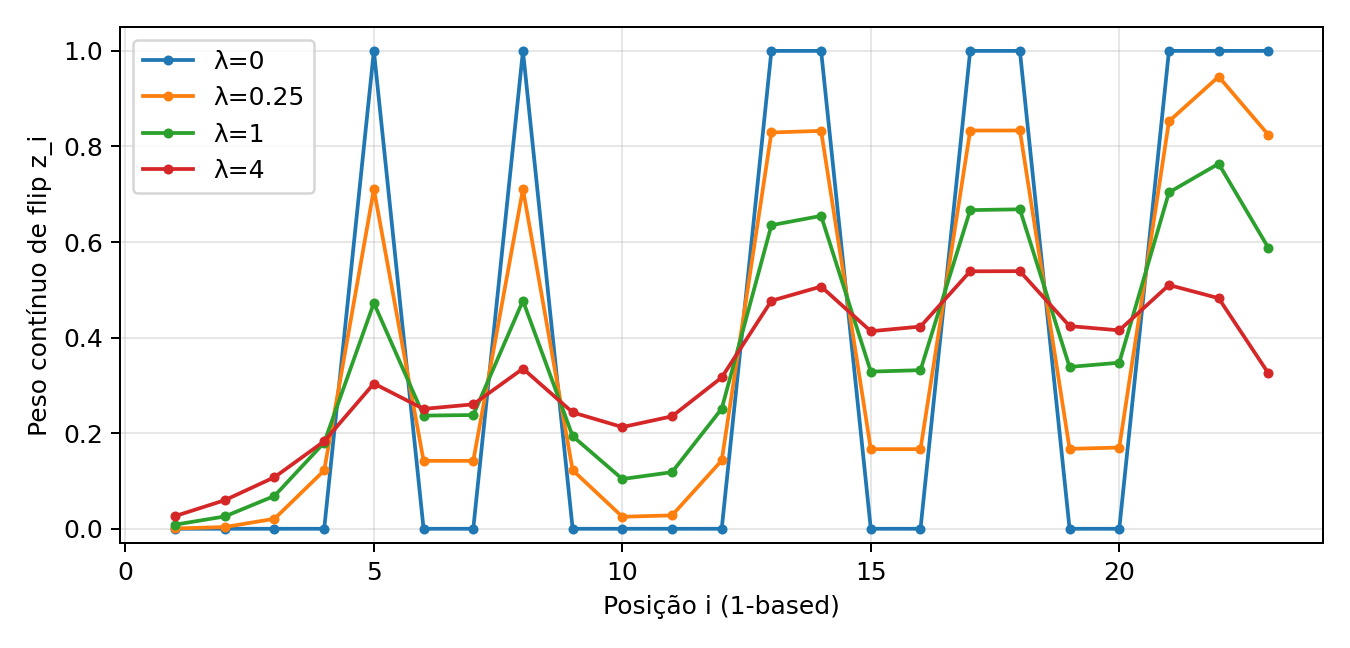
\includegraphics[width=\columnwidth]{resultados/grafico_pesos_flip.png}
\caption{Pesos de alteração por posição para diferentes valores de $\lambda$.}
\label{fig:pesos}
\end{figure}

A trajetória da função objetivo também foi registrada em cada iteração. As execuções apresentaram redução do valor de $J$ até os critérios de parada definidos; esse resultado, contudo, não implica a minimização do número de operações discretas. O gráfico de convergência foi preservado entre os arquivos de resultados do projeto.

\section{Considerações Finais}
A avaliação evidenciou o alto custo da enumeração de estados na BFS e na \textit{Best-First}, em contraste com a exploração direta dos blocos de diferenças. Esta última permitiu obter soluções discretas de custo ótimo até 4096 bits. Na formulação contínua, a penalidade de adjacência reduziu as variações entre posições vizinhas, mas valores elevados de $\lambda$ aumentaram a divergência em relação ao alvo. Portanto, as abordagens atenderam a objetivos distintos: minimizar o número de inversões ou equilibrar fidelidade e regularidade.

A correção das buscas foi conferida em 256 pares de estados de quatro bits; o gradiente também foi verificado por diferenças finitas. Os códigos, as tabelas e os gráficos estão disponíveis no \href{https://github.com/LuanDinizMR/mini-projeto-buscas-otimizacao-IA-0}{repositório GitHub}. Para reproduzir a execução completa, foi utilizado o seguinte comando no terminal, a partir da pasta principal do projeto:
\begin{center}
\verb|python main.py --todos|
\end{center}

\end{document}
